\documentclass[11pt]{article}

\usepackage[margin=1in]{geometry}
\usepackage{amsmath}
\usepackage{amssymb}
\usepackage{amsthm}
\usepackage{enumitem}
\usepackage{tikz}

\newtheoremstyle{solstyle}{6pt}{6pt}{}{}{\bfseries}{.}{ }{}
\theoremstyle{solstyle}
\newtheorem*{solution}{Solution}

\tikzset{v/.style={circle,fill=black,inner sep=1.5pt}}

\newcommand{\glabel}[1]{\begin{center}\textbf{[Graph #1]}\end{center}}

\setlength{\parindent}{0pt}
\setlength{\parskip}{6pt}

\begin{document}

\noindent\textbf{DJ BAAAA}\hfill\textbf{Jul 20, 2026}

\noindent\textbf{Clarifier:} James\\
\textbf{Manager:} Benjamin\\
\textbf{Reporter:} Aaron\\
\textbf{Skeptic:} Daniel

\textbf{Report:} I think most of the problems were solved well. We did spend a bit more time on 5 wondering how to put the proof cleanly into logical text. We also had trouble with 10 because we assumed the largest vertex(s) would connect to all the other largest vertices. We ended up generalizing the argument to provide a reasonable proof. Everything else went well. 

\begin{center}\rule{0.6\textwidth}{0.4pt}\end{center}

\textbf{SOLUTIONS \& PROOFS:}

\begin{enumerate}[leftmargin=*]

\item Find a graph $G$ with order $6$ and size $7$ s.t. $G$ contains no $4$-cycles.

\begin{solution}
Take the $6$-cycle $v_1 \cdots v_6$ and add the single edge $v_4 v_6$.
\end{solution}

\begin{center}
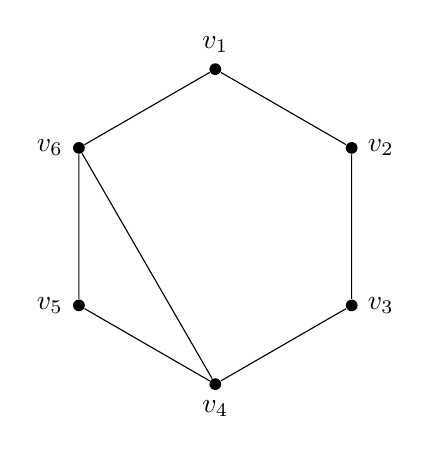
\begin{tikzpicture}
\node[v,label=above:{$v_1$}] (v1) at (90:2) {};
\node[v,label=right:{$v_2$}] (v2) at (30:2) {};
\node[v,label=right:{$v_3$}] (v3) at (-30:2) {};
\node[v,label=below:{$v_4$}] (v4) at (-90:2) {};
\node[v,label=left:{$v_5$}] (v5) at (-150:2) {};
\node[v,label=left:{$v_6$}] (v6) at (150:2) {};
\draw (v1)--(v2)--(v3)--(v4)--(v5)--(v6)--(v1);
\draw (v4)--(v6);
\end{tikzpicture}
\end{center}
\glabel{I}

This graph has order $6$ and size $7$. The edge $v_4 v_6$ splits the hexagon into a triangle $v_4 v_5 v_6$ and a $5$-cycle $v_6 v_1 v_2 v_3 v_4$. The only cycles present have lengths $3$, $5$, and $6$, so there is no $4$-cycle.

\item Isomorphism exercises

\begin{enumerate}[label=(\alph*),leftmargin=*]

\item Prove that the following two graphs ([Graph II] \& [Graph III]) are isomorphic.

\begin{center}
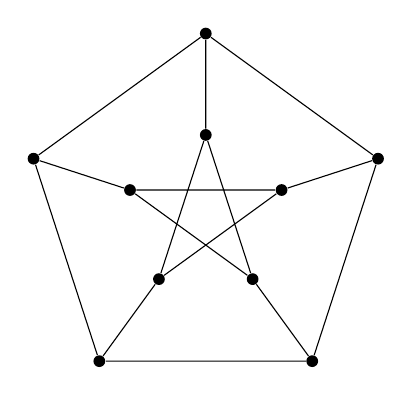
\begin{tikzpicture}[scale=0.92]
\node[v] (A1) at (90:2.5){};
\node[v] (A2) at (18:2.5){};
\node[v] (A3) at (-54:2.5){};
\node[v] (A4) at (-126:2.5){};
\node[v] (A5) at (162:2.5){};
\node[v] (A6) at (90:1.1){};
\node[v] (A7) at (18:1.1){};
\node[v] (A8) at (-54:1.1){};
\node[v] (A9) at (-126:1.1){};
\node[v] (A10) at (162:1.1){};
\draw (A1)--(A2)--(A3)--(A4)--(A5)--(A1);
\draw (A1)--(A6) (A2)--(A7) (A3)--(A8) (A4)--(A9) (A5)--(A10);
\draw (A6)--(A8)--(A10)--(A7)--(A9)--(A6);
\end{tikzpicture}
\qquad
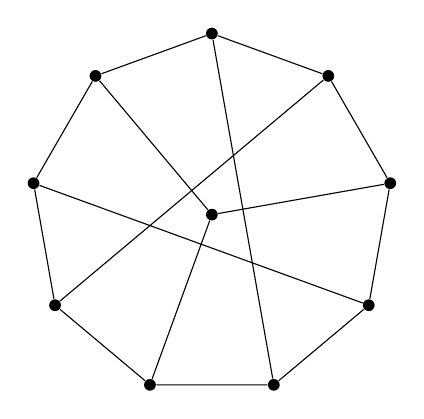
\begin{tikzpicture}[scale=0.92]
\node[v] (A1) at (130:2.5){};
\node[v] (A2) at (90:2.5){};
\node[v] (A3) at (50:2.5){};
\node[v] (A8) at (10:2.5){};
\node[v] (A10) at (-30:2.5){};
\node[v] (A7) at (-70:2.5){};
\node[v] (A9) at (-110:2.5){};
\node[v] (A4) at (-150:2.5){};
\node[v] (A5) at (170:2.5){};
\node[v] (A6) at (0,0){};
\draw (A1)--(A2)--(A3)--(A8)--(A10)--(A7)--(A9)--(A4)--(A5)--(A1);
\draw (A2)--(A7) (A5)--(A10) (A4)--(A3);
\draw (A6)--(A1) (A6)--(A8) (A6)--(A9);
\end{tikzpicture}
\end{center}
\begin{center}\textbf{[Graph II]} \qquad\qquad \textbf{[Graph III]}\end{center}

We redraw the same two graphs with vertex labels, as Graph IV and Graph V, so that we can compare their edges directly.

\begin{center}
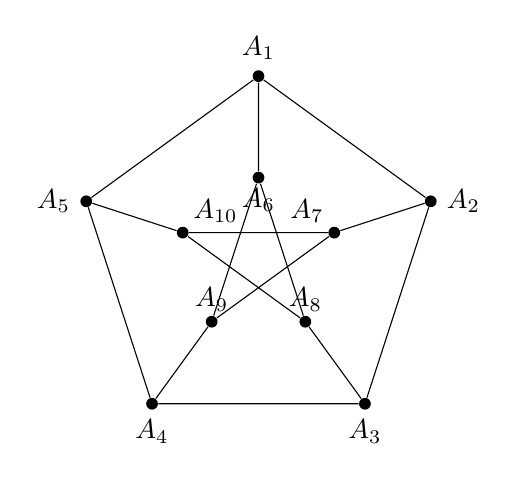
\begin{tikzpicture}[scale=0.92]
\node[v,label=above:{$A_1$}] (A1) at (90:2.5){};
\node[v,label=right:{$A_2$}] (A2) at (18:2.5){};
\node[v,label=below:{$A_3$}] (A3) at (-54:2.5){};
\node[v,label=below:{$A_4$}] (A4) at (-126:2.5){};
\node[v,label=left:{$A_5$}] (A5) at (162:2.5){};
\node[v,label={[label distance=-2pt]-90:{$A_6$}}] (A6) at (90:1.1){};
\node[v,label={[label distance=-2pt]162:{$A_7$}}] (A7) at (18:1.1){};
\node[v,label={[label distance=-2pt]90:{$A_8$}}] (A8) at (-54:1.1){};
\node[v,label={[label distance=-2pt]90:{$A_9$}}] (A9) at (-126:1.1){};
\node[v,label={[label distance=-2pt]18:{$A_{10}$}}] (A10) at (162:1.1){};
\draw (A1)--(A2)--(A3)--(A4)--(A5)--(A1);
\draw (A1)--(A6) (A2)--(A7) (A3)--(A8) (A4)--(A9) (A5)--(A10);
\draw (A6)--(A8)--(A10)--(A7)--(A9)--(A6);
\end{tikzpicture}
\qquad
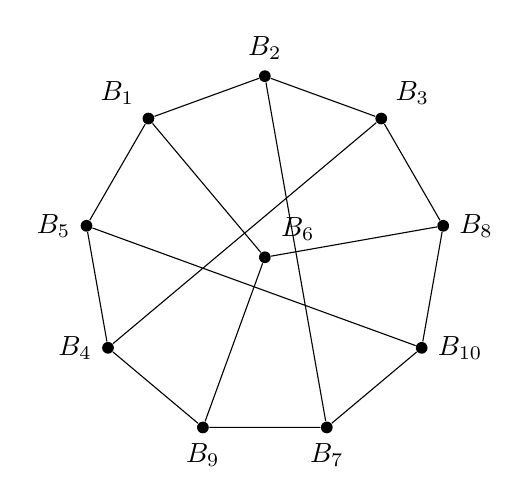
\begin{tikzpicture}[scale=0.92]
\node[v,label=above left:{$B_1$}] (B1) at (130:2.5){};
\node[v,label=above:{$B_2$}] (B2) at (90:2.5){};
\node[v,label=above right:{$B_3$}] (B3) at (50:2.5){};
\node[v,label=right:{$B_8$}] (B8) at (10:2.5){};
\node[v,label=right:{$B_{10}$}] (B10) at (-30:2.5){};
\node[v,label=below:{$B_7$}] (B7) at (-70:2.5){};
\node[v,label=below:{$B_9$}] (B9) at (-110:2.5){};
\node[v,label=left:{$B_4$}] (B4) at (-150:2.5){};
\node[v,label=left:{$B_5$}] (B5) at (170:2.5){};
\node[v,label={[label distance=1pt]45:{$B_6$}}] (B6) at (0,0){};
\draw (B1)--(B2)--(B3)--(B8)--(B10)--(B7)--(B9)--(B4)--(B5)--(B1);
\draw (B2)--(B7) (B5)--(B10) (B4)--(B3);
\draw (B6)--(B1) (B6)--(B8) (B6)--(B9);
\end{tikzpicture}
\end{center}
\begin{center}\textbf{[Graph IV]} \qquad\qquad \textbf{[Graph V]}\end{center}

\begin{proof}
Graph IV and Graph V are each labeled under $A_1,\dots,A_{10}$ and $B_1,\dots,B_{10}$, respectively, so for the two graphs to be isomorphic, there must exist a one-to-one function $\varphi$ such that  $\varphi(A_i)=B_i$. We have defined $B_i$ in a way that $\varphi(x)=x$ suffices the condition. Since the function sends every edge of Graph IV to an edge of Graph V and vice versa, it is an isomorphism.
\end{proof}

\item Prove that the following two graphs ([Graph VI] \& [Graph VII]) are \emph{not} isomorphic.

\begin{center}
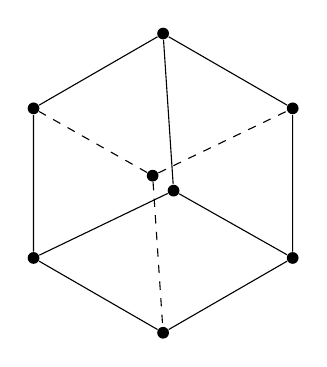
\begin{tikzpicture}[scale=0.95]
\node[v] (v1) at (90:2){};
\node[v] (v2) at (30:2){};
\node[v] (v3) at (-30:2){};
\node[v] (v4) at (-90:2){};
\node[v] (v5) at (-150:2){};
\node[v] (v6) at (150:2){};
\node[v] (n) at (0.14,-0.10){};
\node[v] (f) at (-0.14,0.10){};
\draw (v1)--(v2)--(v3)--(v4)--(v5)--(v6)--(v1);
\draw (n)--(v1) (n)--(v3) (n)--(v5);
\draw[dashed] (f)--(v2) (f)--(v4) (f)--(v6);
\end{tikzpicture}
\qquad
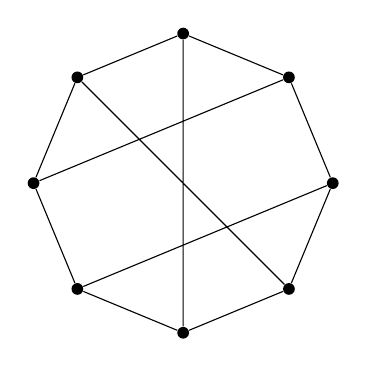
\begin{tikzpicture}[scale=0.95]
\node[v] (w1) at (90:2){};
\node[v] (w2) at (45:2){};
\node[v] (w3) at (0:2){};
\node[v] (w4) at (-45:2){};
\node[v] (w5) at (-90:2){};
\node[v] (w6) at (-135:2){};
\node[v] (w7) at (180:2){};
\node[v] (w8) at (135:2){};
\draw (w1)--(w2)--(w3)--(w4)--(w5)--(w6)--(w7)--(w8)--(w1);
\draw (w1)--(w5) (w2)--(w7) (w3)--(w6) (w4)--(w8);
\end{tikzpicture}
\end{center}
\begin{center}\textbf{[Graph VI]} \qquad\qquad \textbf{[Graph VII]}\end{center}

\begin{proof}
Both graphs are $3$-regular on $8$ vertices, so degrees will not tell them apart. We use cycle lengths instead, which an isomorphism must preserve.

Graph VII has an odd cycle: $w_1 w_2 w_3 w_4 w_5 w_1$, made of four rim edges and the edge $w_5 w_1$, of length $5$. On the contrary, Graph VI has no odd cycle. We can show this by color-coding and path parity.

Color the near corner and $v_2,v_4,v_6$ red, and the far corner and $v_1,v_3,v_5$ blue, as shown in Graph VIII.

\begin{center}
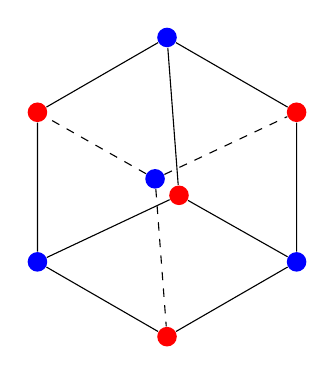
\begin{tikzpicture}[scale=0.95]
\node[v,fill=blue,inner sep=2.5pt] (v1) at (90:2){};
\node[v,fill=red,inner sep=2.5pt] (v2) at (30:2){};
\node[v,fill=blue,inner sep=2.5pt] (v3) at (-30:2){};
\node[v,fill=red,inner sep=2.5pt] (v4) at (-90:2){};
\node[v,fill=blue,inner sep=2.5pt] (v5) at (-150:2){};
\node[v,fill=red,inner sep=2.5pt] (v6) at (150:2){};
\node[v,fill=red,inner sep=2.5pt] (n) at (0.16,-0.11){};
\node[v,fill=blue,inner sep=2.5pt] (f) at (-0.16,0.11){};
\draw (v1)--(v2)--(v3)--(v4)--(v5)--(v6)--(v1);
\draw (n)--(v1) (n)--(v3) (n)--(v5);
\draw[dashed] (f)--(v2) (f)--(v4) (f)--(v6);
\end{tikzpicture}
\end{center}
\glabel{VIII}

Checking the six rim edges and the six edges at the two corners, every edge joins a red vertex to a blue one. Walking along any cycle the color flips at each step, so returning to the start takes an even number of steps. Hence every cycle in Graph VI has even length.

Thus, since Graph VII has a $5$-cycle and Graph VI cannot, the two graphs are not isomorphic.
\end{proof}
\end{enumerate}

\item Recall that the \emph{distance} between two vertices is the length of the shortest path between them. The \emph{diameter} of a graph is the longest distance between two vertices. For example, in [Graph IX], the distance between vertex $A$ and vertex $B$ is $2$, and the diameter of the graph is $3$.

\begin{center}
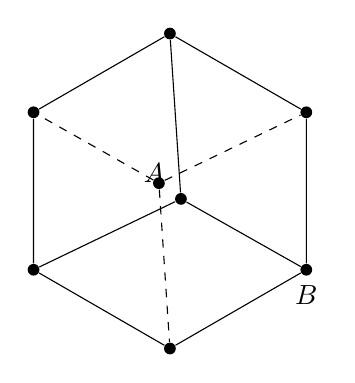
\begin{tikzpicture}[scale=1.0]
\node[v] (v1) at (90:2){};
\node[v] (v2) at (30:2){};
\node[v,label=below:{$B$}] (v3) at (-30:2){};
\node[v] (v4) at (-90:2){};
\node[v] (v5) at (-150:2){};
\node[v] (v6) at (150:2){};
\node[v,label={[label distance=1pt]135:{$A$}}] (n) at (0.14,-0.10){};
\node[v] (f) at (-0.14,0.10){};
\draw (v1)--(v2)--(v3)--(v4)--(v5)--(v6)--(v1);
\draw (n)--(v1) (n)--(v3) (n)--(v5);
\draw[dashed] (f)--(v2) (f)--(v4) (f)--(v6);
\end{tikzpicture}
\end{center}
\glabel{IX}

\begin{enumerate}[label=(\alph*),leftmargin=*]

\item Draw a graph with order $5$ and diameter $1$.

\begin{solution}
The complete graph $K_5$ works.
\end{solution}

\begin{center}
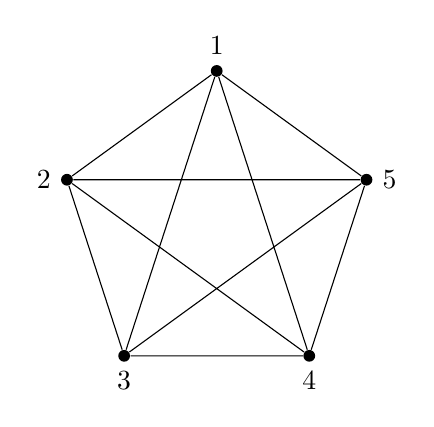
\begin{tikzpicture}
\node[v,label=above:{$1$}] (p1) at (90:2){};
\node[v,label=left:{$2$}] (p2) at (162:2){};
\node[v,label=below:{$3$}] (p3) at (234:2){};
\node[v,label=below:{$4$}] (p4) at (306:2){};
\node[v,label=right:{$5$}] (p5) at (18:2){};
\draw (p1)--(p2)--(p3)--(p4)--(p5)--(p1);
\draw (p1)--(p3) (p1)--(p4) (p2)--(p4) (p2)--(p5) (p3)--(p5);
\end{tikzpicture}
\end{center}
\glabel{X}

\item Draw a graph with order $5$ and diameter $2$.

\begin{solution}
The $5$-cycle with one added edge works.
\end{solution}

\begin{center}
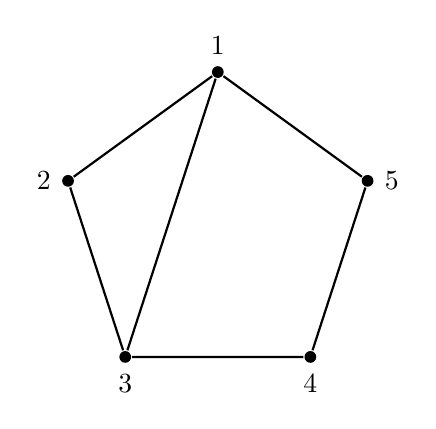
\begin{tikzpicture}[thick]
\node[v,label=above:{$1$}] (p1) at (90:2){};
\node[v,label=left:{$2$}] (p2) at (162:2){};
\node[v,label=below:{$3$}] (p3) at (234:2){};
\node[v,label=below:{$4$}] (p4) at (306:2){};
\node[v,label=right:{$5$}] (p5) at (18:2){};
\draw (p1)--(p2)--(p3)--(p4)--(p5)--(p1);
\draw (p1)--(p3);
\end{tikzpicture}
\end{center}
\glabel{XI}

\item Draw a graph with order $5$ and diameter $3$.

\begin{solution}
A triangle with a path of length $2$ attached to one corner works.
\end{solution}

\begin{center}
\begin{tikzpicture}
\node[v,label=left:{$a$}] (a) at (-0.9,1.6){};
\node[v,label=right:{$b$}] (b) at (0.9,1.6){};
\node[v,label=above:{$c$}] (c) at (0,2.8){};
\node[v,label=left:{$d$}] (d) at (-0.9,0.2){};
\node[v,label=left:{$e$}] (e) at (-0.9,-1.2){};
\draw (a)--(b)--(c)--(a);
\draw (a)--(d)--(e);
\end{tikzpicture}
\end{center}
\glabel{XII}

\item Try to categorize the graphs of diameter $1$.

\begin{solution}
Exactly the complete graphs $K_n$ with $n\ge 2$.
\end{solution}

\begin{proof}
Diameter $1$ means every two distinct vertices are at distance $1$, that is, adjacent. That is exactly the definition of $K_n$, so these are the complete graphs. We need $n\ge 2$, since $K_1$ has diameter $0$.
\end{proof}

\end{enumerate}

\item Find the size of $K_n$.

\begin{solution}
The size of $K_n$ is $\dbinom{n}{2}=\dfrac{n(n-1)}{2}$.
\end{solution}

\begin{proof}
Every vertex of $K_n$ has degree $n-1$, so the degree sum is $n(n-1)$. By the degree-sum formula this equals $2\lvert E\rvert$, hence $\lvert E\rvert = \dfrac{n(n-1)}{2}=\dbinom{n}{2}$.
\end{proof}

\item We've never precisely defined ``cycle'' although we've talked about it. A \emph{cycle} is a sequence of vertices, each a neighbor of the previous one, that ends where it began, and no vertex is repeated, excluding the first and last one. In other words a ``cycle'' is like a path where the first and last vertices are the same vertex. Let $G$ be a graph. Prove that if every vertex of $G$ has degree at least $2$, then $G$ contains a cycle.

\begin{proof}
Take a longest path $P: v_0 v_1 \cdots v_k$ in $G$, which exists because $G$ is finite. Since $\deg(v_0)\ge 2$, the endpoint $v_0$ has a neighbor $u\ne v_1$. If $u$ were not on $P$, then $u\,v_0\,v_1\cdots v_k$ would be a longer path, contradiction. So $u=v_i$ for some $i\ge 2$, and $v_0 v_1 \cdots v_i v_0$ is a cycle.
\end{proof}

\item Let $G$ be a general graph with exactly two vertices $x$ and $y$ of odd degree (the rest of the vertices are even degreed). Let $G^{*}$ be the general graph obtained by putting a new edge $\{x,y\}$ joining $x$ and $y$. Prove that $G$ is connected IFF $G^{*}$ is connected.

\begin{proof}

($\Rightarrow$) $G$ is a subgraph of $G^{*}$, so if $G$ is connected every pair of vertices is still joined by a path in $G^{*}$, and therefore $G^{*}$ is connected.

($\Leftarrow$) Suppose $G^{*}$ is connected but $G$ is not. Removing one edge from a connected graph splits it into at most two pieces, so $G$ has exactly two components, with $x$ and $y$ in different ones (otherwise deleting $xy$ would not disconnect $G^{*}$). The component containing $x$ then has $x$ as its only odd-degree vertex, since $y$ is not in it. But every graph has an even number of odd-degree vertices, so this is impossible. Hence $G$ is connected.
\end{proof}

\item Is it true that a finite graph having exactly two vertices of odd degree must contain a path from one to the other? Give a proof or a counterexample.

\begin{proof}  
For a connected graph $G$ that contains $2$ vertices of odd degree, by the definition of a connected graph, there must be a path from one vertex of odd degree to the other vertex of odd degree.

For a disconnected graph $G$ with some number of components, we focus on two components. Component 1 has a vertex $A$ of odd degree attached to a connected graph $G_A$. Component 2 has a vertex $B$ of odd degree attached to a connected graph $G_B$. Let the graph containing components 1 and 2 be $H$. From the results of problem 6, $H$ is connected iff $H^{*}$ is connected, where $H^{*}$ is the graph that connects vertices $A$ and $B$. However, because $G$ is disconnected, this means that while graph $H$ is connected, meaning there must be a path between $A$ and $B$ even though $G$ is disconnected, some other component of $G$ is disconnected, in which it must have vertices that all have even degree via the restriction in the problem.
\end{proof}

\item How many $3$-regular graphs are there of order $11$? Prove that you have found them all.
\begin{solution}
None. 
\end{solution}
\begin{proof}
Such a graph would have degree sum $3\cdot 11=33$, which is odd, but the degree sum always equals $2\lvert E\rvert$, an even number.
\end{proof}

\item \textbf{[CHALLENGE]} Find a $3$-regular graph of diameter $2$ with the largest order you can. You don't have to prove your result is the largest possible.

\begin{solution}
The largest possible order is $10$, achieved by the following graph (Graph XIII).
\end{solution}

\begin{center}
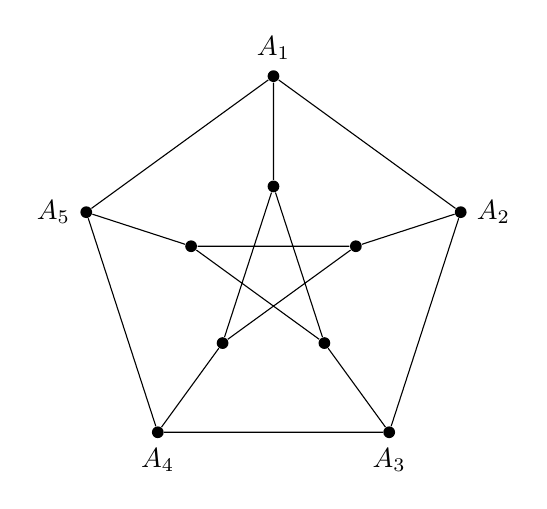
\begin{tikzpicture}
\node[v,label=above:{$A_1$}] (A1) at (90:2.5){};
\node[v,label=right:{$A_2$}] (A2) at (18:2.5){};
\node[v,label=below:{$A_3$}] (A3) at (-54:2.5){};
\node[v,label=below:{$A_4$}] (A4) at (-126:2.5){};
\node[v,label=left:{$A_5$}] (A5) at (162:2.5){};
\node[v] (A6) at (90:1.1){};
\node[v] (A7) at (18:1.1){};
\node[v] (A8) at (-54:1.1){};
\node[v] (A9) at (-126:1.1){};
\node[v] (A10) at (162:1.1){};
\draw (A1)--(A2)--(A3)--(A4)--(A5)--(A1);
\draw (A1)--(A6) (A2)--(A7) (A3)--(A8) (A4)--(A9) (A5)--(A10);
\draw (A6)--(A8)--(A10)--(A7)--(A9)--(A6);
\end{tikzpicture}
\end{center}
\glabel{XIII}

\begin{proof}
Fix a vertex $u$. It has $3$ neighbors, and each neighbor has at most $2$ other neighbors, so with diameter $2$ every vertex is $u$, a neighbor, or a neighbor of a neighbor: at most $1+3+3\cdot 2=10$ vertices. Graph XIII is $3$-regular with diameter $2$ on exactly $10$ vertices, so the bound is attained.
\end{proof}

\item \textbf{[CHALLENGE]} If a non-increasing sequence of numbers can serve as the degree sequence of some graph, it is called a \emph{graphic sequence}. For example, this is a graphic sequence : $\{4, 4, 2, 2, 2, 2\}$.

\begin{enumerate}[label=(\alph*),leftmargin=*]

\item Prove that if $\{t_1-1,\; t_2-1,\; \cdots\; t_s-1,\; d_1,\; \cdots\; d_p\}$ is a graphic sequence, then so is $\{s,\; t_1,\; t_2,\; \cdots\; t_s,\; d_1,\; \cdots\; d_p\}$.

\begin{proof}
Take a graph $H$ sufficing the reduced sequence, with vertices $u_1,\dots,u_s$ of degrees $t_1-1,\dots,t_s-1$. Add one new vertex $w$ and join it to $u_1,\dots,u_s$. Then $w$ has degree $s$, each $u_i$ rises to degree $t_i$, and the $d_j$ vertices are unchanged, so the longer sequence is graphic.
\end{proof}

\item Prove that if $\{s,\; t_1,\; t_2,\; \cdots\; t_s,\; d_1,\; \cdots\; d_p\}$ is a graphic sequence, then so is $\{t_1-1,\; t_2-1,\; \cdots\; t_s-1,\; d_1,\; \cdots\; d_p\}$.

\begin{proof}
Among all graphs sufficing the graphic sequence $s, t_1, \dots, t_s, d_1, \dots, d_p$, let $w$ be a vertex of degree $s$, and without loss of generality(WLoG) pick the case that maximizes the sum of the degrees of $w$'s neighbors.

Proof of Generality: We claim $w$ is joined to the $s$ vertices of largest degree, namely those of degrees $t_1,\dots,t_s$. If not, there are vertices $a\notin N(w)$ and $b\in N(w)$ with $\deg(a)>\deg(b)$. Since $\deg(a)>\deg(b)$ and $w\in N(b)\setminus N(a)$, there is some $c\in N(a)\setminus N(b)$ with $c\ne w,b$. Delete the edges $wb$ and $ac$ and add $wa$ and $bc$. All degrees stay the same, but $w$ has swapped its neighbor $b$ for the higher-degree $a$, raising the neighbor-degree sum, contradicting maximality.

So $w$ is joined exactly to the vertices of degrees $t_1,\dots,t_s$. Deleting $w$ lowers each of those by $1$, leaving a graph with degrees $t_1-1,\dots,t_s-1,d_1,\dots,d_p$. Hence the reduced sequence is graphic.
\end{proof}

\end{enumerate}

\end{enumerate}

\end{document}